\documentclass{article}
\usepackage[utf8]{inputenc}
\usepackage{a4wide,parskip,underscore,xspace,graphicx}
\usepackage{minted}
\usepackage{hyperref}
\hypersetup{
    colorlinks=true,
    linkcolor=blue,
    urlcolor=blue,
    citecolor=black
}

\newcommand*{\mono}[1]{\texttt{#1}}
% \newcommand*{\code}[1]{\texttt{#1}}
\newcommand*{\code}[1]{\mintinline{julia}{#1}}
\newcommand*{\TODO}{\textbf{TODO}\xspace}

\title{Digital Signal Processing - Assignment 4a}
\author{Joshua Perrett (jdp63)}
\date{January 2023}

\begin{document}

\maketitle

\section*{Introduction}

For the mini-project, I opted for the first option: ``HDMI video cable eavesdropping''. The steps provided are quite clear, and so I will describe my results more or less in the order that corresponds to the instructions given.

My full work is available here (to be made public shortly after the submission deadline): \\ https://github.com/jperrett256/UOC2022-DSP-project



\section*{Resampling}

To display an image, the data needed resampling to some frequency $f_r$ that was a multiple of $f_p$ (to have an integer number of samples per line). I found $fr = f_p$ to result in a poor quality image, while $fr = 2 * f_p$ (or above) worked fine. This implies that highest frequencies in the data were around $f_p$ (using the Nyquist criterion).

I initially tried performing perfect sinc interpolation (see code below), which worked fine for a test input, but took far too long on the IQ data (even for just a couple of frames).

% TODO show perfect sinc interpolation code
\begin{minted}{julia}
    function change_fs(old_len, old_ys, old_fs :: Int, new_fs :: Int)
        new_len = floor(Int, old_len * new_fs/old_fs);
        new_xs = collect(0:new_len-1) / new_fs;

        new_ys = zeros(new_len)
        for i=0:old_len-1
          new_ys += old_ys[i+1] * sinc.(old_fs * (new_xs .- (i / old_fs)));
        end

        return new_len, new_xs, new_ys
    end;
\end{minted}


After looking for more computationally-feasible approaches to resampling, I found a resource that implied that changing ``the sampling rate by a rational factor'' required interpolating and then decimating \cite{dspguru-resampling}. If the rational factor has a very large numerator, this process can require a great deal of memory. To mitigate this, the process can be divided into multiple stages, by splitting the factor into a series of smaller factors with smaller numerators and denominators \cite{dspguru-resampling}. This seemed surprisingly complicated for such a core operation, but it appears (from reading the source code) that the Julia DSP library uses this method exactly \cite{dsp-julia-github}. The \code{resample} function uses a Kaiser filter (unless explicitly supplied with one in the function arguments) \cite{dsp-julia-github}. (The important files to look at are \code{src/Filters/stream_filt.jl} and \mono{src/Filters/design.jl}.)

\begin{minted}{julia}
    fr = 2 * fp;
    fs = MHz(64); # MHz(x) is my function, just multiplies its input by 10^6
    z_resampled = resample(z, fr/fs);
\end{minted}

\section*{Parameter Values}

Adjusting by eye, I found that $f_p$ was +0.1\% over the expected 25.175 MHz. By vertically joining two separate frames that were several frames apart, I updated my estimate to +0.0997\%.

After fixing the alignment (by discarding samples), this yielded the result seen in Figure \ref{fig:grayscale-image}.

I managed to produce all my images using the \code{heatmap} function:
\begin{minted}{julia}
    function plot_image(img :: AbstractMatrix; aspectratio=1 :: Real)
        heatmap(img, aspectratio=aspectratio, yflip=true,
            colorbar=:none, axis=([], false), color=cgrad(:grays));
    end;
\end{minted}

\subsection*{Using Autocorrelation for Automatic Adjustment}

\begin{figure}
    \centering
    \includegraphics[width=0.8\linewidth]{images/grayscale_manually_tuned_2_frames_joined.png}
    \caption{Result from manually tuning $f_p$ and setting the alignment. Top half is the first frame, bottom half is the last frame. (Note that the automatically tuned version looks identical.)}
    \label{fig:grayscale-image}
\end{figure}

\begin{figure}
    \centering
    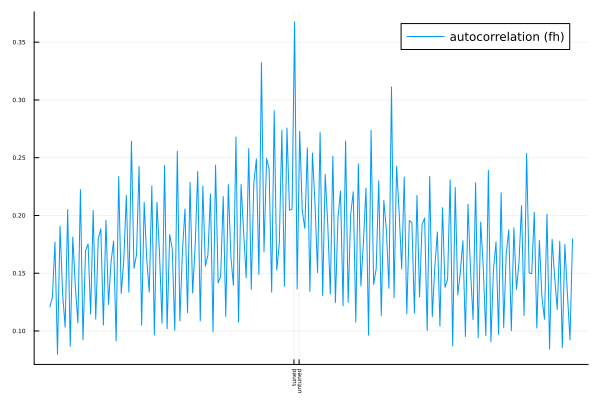
\includegraphics[width=\linewidth]{images/autocor_fh.png}
    \caption{The labels say ``tuned'' and ``untuned'', where ``tuned'' refers to the manual estimate, and ``untuned'' refers to the case where $f_p$ is exactly 25.175 MHz. There is a large spike more or less exactly where the manual estimate was.}
    \label{fig:autocorrelation-fh}
\end{figure}

In order to automate the estimation of $f_p$, the \code{StatsBase.autocor} function was used to compute autocorrelation. The $k$th value of the autocorrelation function gives you the sum of all products of values in the sequence that are a distance $k$ apart. The second parameter of \code{StatsBase.autocor} specifies the range of values for $k$, and choosing a suitable range is important for bounding the execution time.

If we have $f_h$ tuned perfectly, then samples that are $f_s/f_h$ apart correspond to data immediately above or below in the image. Given the horizontal blank for each row is presumably the same predictable pattern, multiplying them will produce a large number, and we can expect a spike in the autocorrelation.

(All the same can be said for $f_v$, with samples that are $f_s/f_v$ apart, because of the vertical blanking interval.)

We can use this fact to estimate $f_h$ or $f_v$, which will in turn give us an estimate of $f_p$. To keep the execution time reasonable, the following code finds upper and lower bounds for $f_h$ and $f_v$ given $f_p = \textnormal{25.175 MHz} \pm \textnormal{0.5\%}$ and computes the autocorrelation for values of $k$ in the ranges corresponding to these bounds.

\begin{minted}{julia}
    using StatsBase;

    function get_freqs(fp)
        fh = fp/xt;
        fv = fh/yt;
        return fh, fv;
    end;

    # assumes no deviation from 25.175 MHz
    fp_std = fp_standard;
    fh_std, fv_std = get_freqs(fp_std);

    # manually tuned values
    fp_ref = round(Int, fp_std * 1.000997); # +-0.5% range
    fh_ref, fv_ref = get_freqs(fp_ref);

    # upper and lower bounds
    fp_low = floor(Int, fp_std * 0.95);
    fh_low, fv_low = get_freqs(fp_low);
    fp_high = ceil(Int, fp_std * 1.05);
    fh_high, fv_high = get_freqs(fp_high);

    autocor_fh = autocor(abs.(z), xs_fh);
    autocor_fv = autocor(abs.(z), xs_fv); # SLOW

    plot(xs_fh, autocor_fh;
        xticks=([fs/fh_ref, fs/fh_std], ["tuned", "untuned"]),
        xrotation=90, tickfontsize=4, dpi=300, label="autocorrelation (fh)");
    # can similarly plot autocor_fv
\end{minted}

The above results in the graph shown in Figure \ref{fig:autocorrelation-fh}. One concern is that the graph is rather noisy, and a different peak could be mistaken for the peak we are looking for. It is possible that smoothing the graph by applying a Gaussian kernel could be an effective strategy for avoiding issues, though more testing would be needed to validate this claim. In our case, smoothing the graph does not change where the maximum is located. The code for doing this is below, and the smoothed graph can be seen in Figure \ref{fig:autocorrelation-fh-smooth}.

\begin{minted}{julia}
    ker = ImageFiltering.Kernel.gaussian((3,));
    autocor_fh_filtered = imfilter(autocor_fh, ker);

    # In our case, these two print statements print the same thing.

    # finds value of k corresponding to maximum in original graph
    println(xs_fh[findmax(autocor_fh)[2]]);
    # finds value of k corresponding to maximum in smooth graph
    println(xs_fh[findmax(autocor_fh_filtered)[2]]);


    plot(xs_fh, autocor_fh_filtered;
        xticks=([fs/fh_ref, fs/fh_std], ["tuned", "untuned"]),
        xrotation=90, tickfontsize=4, dpi=300, label="autocorrelation (fh)");
\end{minted}

\begin{figure}
    \centering
    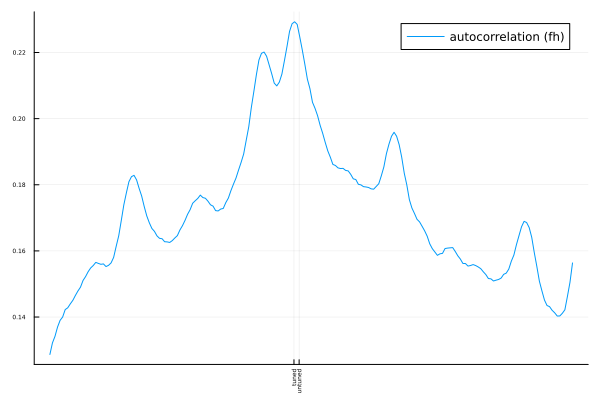
\includegraphics[width=\linewidth]{images/autocor_fh_smooth.png}
    \caption{This is the same data from Figure \ref{fig:autocorrelation-fh}, smoothed with a Gaussian filter. There is still a large peak more or less exactly where the manual estimate was.}
    \label{fig:autocorrelation-fh-smooth}
\end{figure}

The exact same process can be done with $f_v$, and a graph of \code{autocor_fv} is shown in Figure \ref{fig:autocorrelation-fv}. Calculating \code{autocor_fv} takes much longer than \code{autocor_fh}, as the bounds for $k$ are much larger (the distance between pixels in consecutive frames varies wildly with small changes in $f_p$). I did not have as much success applying a Gaussian to this graph.

\begin{figure}
    \centering
    \includegraphics[width=\linewidth]{images/hi_res_autocor_fv.png}
    \caption{The labels say ``tuned'' and ``untuned'', where ``tuned'' refers to the manual estimate, and ``untuned'' refers to the case where $f_p$ is exactly 25.175 MHz. There is a large spike more or less exactly where the manual estimate was.}
    \label{fig:autocorrelation-fv}
\end{figure}

The graphs shown were produced using all of the samples, but a smaller subset can be used. I found that using just two frames worth of samples can produce a graph for \code{autocor_fh} that looks indistinguishable from the graph shown in Figure \ref{fig:autocorrelation-fh}. (This makes some sense, as there are many horizontal blanking intervals in the span of two frames.) Not only is \code{autocor_fv} much slower to compute for a given number of frames, but I found it takes about four frames worth of samples to get a graph that is only very close.

\subsection*{Using Crosscorrelation to Improve Precision}

The main issue with taking estimates from these graphs is the lack of precision. By taking the maximum, we obtain estimates for $f_s / f_h$ and $f_s / f_v$ (from \code{autocor_fh} and \code{autocor_fv} respectively), but these are only to the nearest integer. This limits the precision of the estimates for $f_h$ and $f_v$ (and therefore $f_p$).

It is worth noting that the $f_v$ estimate from \code{autocor_fv} is better than the $f_h$ estimate from \code{autocor_fv}. This is because $f_h$ is much larger than $f_v$, meaning $f_s / f_h$ is much smaller, and so more precision is lost by rounding to the nearest integer. However, even the estimate from $autocor_fv$ appears slightly worse than my manual estimate.

However, we can use crosscorrelation between frames to greatly improve our estimate. (Note that autocorrelation is really just crosscorrelation of a vector with itself. Since the samples for all frames are stored in a single vector, crosscorrelation between frames can be achieved through the same \code{StatsBase.autocor} function.) We expect there to be peaks in the autocorrelation of \code{z} at multiples of $f_s / f_h$ and $f_s / f_v$ as well. If we have an estimate of e.g. $n * f_s / f_h$ that is accurate to the nearest integer, we end up with an estimate of $f_h$ that is much more precise than before. As $n$ increases, we get more precision.

The code below tries to find the crosscorrelation between the first and last frames. We use the previous automatic estimate (by performing autocorrelation within a frame) in order to narrow the bounds of our search, as setting bounds only using the fact that $f_p = \textnormal{25.175 MHz} \pm \textnormal{0.5\%}$ as we did before would result in far too large a range of values for $k$ (the range is multiplied by $n$).

\begin{minted}{julia}
    z = iq_samples;

    # using first automatic estimate of fs/fv
    fs_over_fv_est = xs_fv[findmax(autocor_fv)[2]];
    fs_over_fv_low = fs_over_fv_est - 1;
    fs_over_fv_high = fs_over_fv_est + 1;

    fv_est = fs/fs_over_fv_est;

    est_samples_per_frame = round(Int, fs_over_fv_est);
    min_num_frames = floor(Int, length(z) / est_samples_per_frame);

    xs2_fv = (fs_over_fv_low * min_num_frames):(fs_over_fv_high * min_num_frames);
    xcorr_fv = autocor(abs.(z), xs2_fv);

    fv_est2 = fs * min_num_frames / xs2_fv[findmax(xcorr_fv)[2]];

    println("First automatic estimate: ", fv_est)
    println("Second automatic estimate: ", fv_est2);
    println("Manually tuned estimate: ", fv_ref);

    plot(xs2_fv, xcorr_fv; label="autocorrelation (fv)",
        xticks=([fs/fv_est * xcorr_fv_factor, fs/fv_ref * xcorr_fv_factor],
        ["previous estimate", "hand tuned"]), dpi=300);
\end{minted}

The above results in the graph shown at \ref{fig:xcorr-fv}. This technique allows us to get an estimate that is better than my hand tuned one.

\begin{figure}
    \centering
    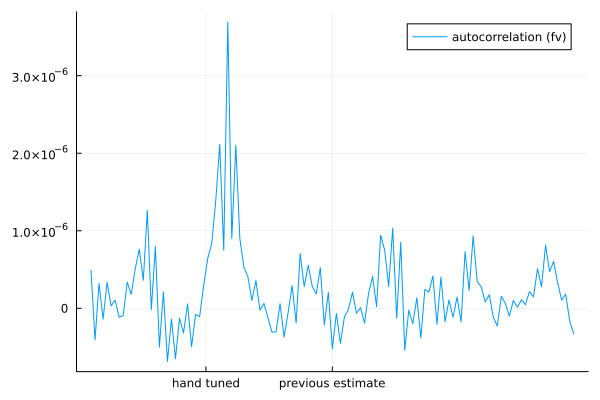
\includegraphics[width=0.95\linewidth]{images/autocor_fv_step2.png}
    \caption{The ``hand tuned'' label refers to the manual estimate, and the ``previous estimate'' label refers to the previous $f_s/f_v$ estimate (from performing autocorrelation). By using the peak on the graph, we can obtain an estimate even better than our original hand tuned one!}
    \label{fig:xcorr-fv}
\end{figure}

The same can be done with $f_h$, using our previous $f_h$ estimate (from performing autocorrelation within a frame). This results in the graph shown at \ref{fig:xcorr-fh}. While this gets us a much better estimate than before (as indicated by it being closer to the hand tuned estimate), using it to resample and display the image shows that it is still a bit off.
\begin{figure}
    \centering
    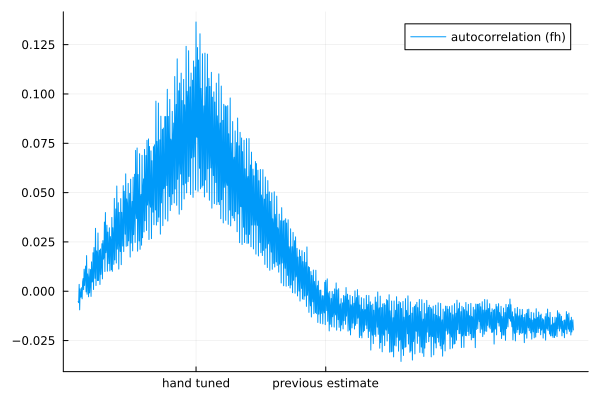
\includegraphics[width=0.95\linewidth]{images/autocor_fh_step2.png}
    \caption{The ``hand tuned'' label refers to the manual estimate, and the ``previous estimate'' label refers to the previous $f_s/f_h$ estimate (from performing autocorrelation).}
    \label{fig:xcorr-fh}
\end{figure}

\section*{Averaging Across Frames}

Figure \ref{fig:grayscale-averaged} shows the grayscale image averaged across frames.

Figure \ref{fig:periodic-phase-spectrogram} shows spectral peaks at $16 \cdot f_p - f_c$ and $17 \cdot f_p - f_c$. I found setting $f_u$ to either of these values worked fine for generating a valid HSV image (before or after resampling to $f_r$). My code for displaying the valid HSV image (shown in Figure \ref{fig:periodic-phase-averaging}) is:

\begin{minted}{julia}
    fv = fv_est2;
    fh = fv * yt;
    fp = fh * xt;

    fc = MHz(425);
    z = iq_samples;

    # fu = 17*fp - fc;
    fu = 16*fp - fc;

    # fc = MHz(400);
    # z = iq_samples_400;
    # fu = 15*fp - fc;

    phasor = cis.(-2\pi * fu / fs .* collect(1:length(z)));
    z = z .* phasor;

    fr = 2 * fp;

    z_resampled = resample(z, fr/fs);
    new_num_samples = min(length(z_resampled), floor(Int, fr / fs * length(z)));
    z_resampled = z_resampled[1:new_num_samples];

    samples_per_line = round(Int, fr/fh);
    samples_per_pixel = round(Int, fr/fp);
    samples_per_frame = round(Int, fr/fv);

    start_idx = 260 * samples_per_line + 450 * samples_per_pixel;
    z_adjusted = z_resampled[start_idx:end];
    num_frames_adjusted = fv * length(z_adjusted) / fr;

    average_img = zeros(ComplexF64, samples_per_frame);
    for i=1:floor(Int,num_frames_adjusted)
        average_img = average_img .+
            z_adjusted[round(Int, fr/fv*(i-1)+1):round(Int, fr/fv*i)];
    end

    average_img /= floor(Int,num_frames_adjusted);

    println("RMS: ", sqrt(1 / length(average_img) * sum(abs2.(average_img))));

    complex_img = reshape(average_img, (samples_per_line, :))';

    # RED-GREEN version
    # r = real.(complex_img);
    # g = imag.(complex_img);
    # @assert size(r) == size(g);

    # # normalise
    # r = r / findmax(r)[1];
    # g = g / findmax(g)[1];

    # imresize(colorview(RGB, r, g, zeros(size(r))), (yt, xt));

    # HSV version
    h = rad2deg.(angle.(complex_img));
    v = abs.(complex_img);
    v = v / findmax(v)[1];

    imresize(colorview(RGB, convert(Matrix{RGB{Float64}},
        HSV.(h, ones(size(h)), v))), (yt, xt));
\end{minted}

\begin{figure}
    \centering
    \includegraphics[width=0.8\linewidth]{images/grayscale_averaged.png}
    \caption{Average of all frames in the recording.}
    \label{fig:grayscale-averaged}
\end{figure}

\begin{figure}
    \centering
    \includegraphics[width=\linewidth]{images/periodic_phase_spectrogram_425.png}
    \caption{Spectrogram for the $f_c = \textnormal{425 MHz}$ IQ sample data.}
    \label{fig:periodic-phase-spectrogram}
\end{figure}

\begin{figure}
    \centering
    \includegraphics[width=\linewidth]{images/periodic_phase_averaging.png}
    \caption{An HSV image produced with periodic phase averaging after phase unrotation.}
    \label{fig:periodic-phase-averaging}
\end{figure}

Periodic averaging without prior phase unrotation yields no image. The RMS for the average of the complex-valued signal without phase unrotation was $3.86 \times 10^{-6}$, with phase unrotation it was $3.78 \times 10^{-5}$. I expected the RMS without unrotation to be small, as summing many random complex values (pointed in all directions) should approach zero. I expected the RMS with phase unrotation to be larger, but the signal may just be very weak. It is an order of magnitude larger.

It appears to be possible to display images using the other IQ recordings, but the result seems to be increasingly noisy and unclear the further away $f_c$ is from 425 MHz.

\section*{Stitching Recordings Together}
I ran out of time for the stitching of 40 MHz recordings, so I will just briefly describe how I would hypothetically do it.

Since each recording is 25 MHz apart, I would stitch five of these together to form a single 125 MHz signal. Each would need resampling to 125 MHz, and then frequency shifting appropriately. Then they would be filtered so that when combined their signals do not overlap. Finally, we just add the signals together (which has the effect of summing their frequency domains), hopefully producing a single valid 125 MHz recording.

Since all three color channels are transmitted simultaneously, it does not seem feasible to expect to read out the data for each colour channel (after decoding TMDS). I expect the result of this would be a clearer HSV image, possibly with enough detail to see the background window clearly.

\section*{Conclusion}

This project was an exciting opportunity to examine HDMI signals, and it was very satisfying to successfully reconstruct HSV images from the IQ data.

\newpage
\appendix
% TODO appendices if needed

\newpage
\bibliographystyle{plain}
\bibliography{refs}

\end{document}
